%%% NEXT CHAPTER #################################################
%##################################################################

\chapter{Source Language Selection}
\label{chap:sourceLanguageSelection}

Bilingual corpora offer a promising bridge between resource-rich and resource-poor languages, enabling the development of multilingual NLP technologies for a far wider range of languages.  In the previous chapter, we used bilingual corpora to build a tagger for the target language. Its performance is on par with the state-of-the-art \cite{Das:2011}. In this chapter we would like to further improve our tagger by investigating source language factors. English is often used as a source language, but it is not the only available
resource-rich language, and another choice may have a dramatic effect
on performance. Where multiple source languages are available, what should we do? How can we combine them? The relationship of source language selection and the universal tagger will be thoroughly considered in this chapter. 

\section{Introduction}

Parallel texts are becoming increasingly available through
sources such as multilingual websites, multilingual documents and large archives of translation memory from books, news. Not only the size but also the number of languages covered by parallel data is increasing. The era of English dominating one side of parallel texts is shifting to a far wider range of languages. Parallel data can be exploited to bridge languages, and in particular, transfer annotated information from a highly-resourced \emph{source} language to a lesser-resourced
\emph{target} language, to build unsupervised POS taggers as demonstrated in Chapter  \ref{chap:uniTagger}. 

One issue in building such a tagger is choosing the source
language. English is commonly used, because parallel data which has
English on one side is often most readily available. However, the
appropriate source language might depend on the target language. 
% Motivation 
Chapter \ref{chap:uniTagger} shows that taggers for languages which are in the same language family tree (Germanic) with source language (English) perform better than the state-of-the-art \cite{Das:2011}. \namecite{SnyderMultilingualPOS} suggested that performance of Slovene tagger improves 7.69\% (absolute) when paired with Serbian, a very closely related language, but only 1.3\% when paired with English. \namecite{reddy2011crosspos} and \namecite{Hana04} show that for closely related languages, the transition probabilities for an HMM tagger can be
used interchangeably.  This experience demonstrates that the choice of
source language might have a drastic effect on target language tagger performance. Moreover, if parallel data for a target language with more than one source language is available, it might be possible to exploit this additional information; however, this issue has not been explored to date. Thus, in this chapter we investigate the problem of making a good choice of source language(s).

% Added overview of paper

In this chapter we are going to build unsupervised POS taggers for $m$ language
pairs using the tagger from chapter \ref{chap:uniTagger}. We identify features --- derived from both monolingual and parallel corpora --- that we could use to predict the best source language to build a tagger for a given target language. We show that choosing an appropriate source language can improve the accuracy of our
state-of-the-art unsupervised POS tagging methodology, compared to
using a single fixed source language. This prediction can be done
based on features of the source and target language derived from
monolingual corpora, although further improvements can be obtained
using the features based on parallel corpora. We then show that even
better accurate prediction can be obtained by incorporating information from
multiple source languages. 

Formally speaking, assuming that we need to build tagger for target language $t$, we have all possible source languages  $s_1,s_2...s_n$. In this chapter, we are going to answer two questions: (1)~what is the best source language $s_i$? (2)~Can we do better by combining multiple source languages? To answer these two questions, we experiment as follows:

%% The first question when building this kind of tagger is choosing the
%% source language. People normally use English as parallel data which
%% has English in one side is easier to acquire. However, is English a
%% good choice? What we should do if we have more than one possible
%% source language. Formally, assuming that we need to build tagger for
%% target language $y$, we have all possible source language
%% $x_1,x_2...x_n$. In this paper, we are trying to answer two questions
%% such that, (1) \textit{``what is the best source language $x_i$?"} (2)
%% \textit{``What if we combine multiple source languages?"}. 

 \begin{enumerate}
 \itemsep0em
 \item Pick $n$ languages  (Section \ref{sec:collectParaData})
 \item Collect $ n \times (n-1)$ parallel data sets (Section \ref{sec:collectParaData})
 \item Define features (Section \ref{featuresSec})
 \item Using parallel data from each language pair, build the tagger (Section \ref{sec:buildTagger})
 \item Build a source language predicting model based on the features (Section \ref{sec:sourceLanguagePrediction})
 \item Combine multiple source languages (Section \ref{sec:multipleSourceLanguages})
 \end{enumerate}

%% Kind of motivation here, I don't think we should move to related work part. 

\section{Collect parallel data}
\label{sec:collectParaData}
We would like to conduct experiments on a resource-poor target language, however, it would be much harder to evaluate. We instead experiment with the same $n = 9$ languages (English, Danish, Dutch, Portuguese, Swedish, Greek, Italian, German, Spanish).  We use the JRC-Acquis corpus which provides parallel data for every pair of 22 European languages~\cite{SteinbergerAcquis}. We thus, extract a subset of 72 language pairs. It's worth noting that we consider ($x-y$) and ($y-x$) to be two different language pairs. 

JRC-Acquis contains of EU legislation, rights, agreements, declarations etc that must be translated to all participating EU countries (currently 22). Thus, theoretically, each document would have a translation into 21 other languages. However, many documents for some languages are unavailable. Only documents that have translation into at least 10 other languages are included in the JRC-Acquis corpus. 

To the best of our knowledge, JRC-Acquis is the biggest corpus providing parallel data for all of the language pairs we consider. Table~\ref{tab:acquis} shows some monolingual statistics about each language. Table \ref{tab:jrcAcquisSizeEachPair} shows the size of parallel data (number of sentences) for each language pair. It is clear that, parallel data in JRC-Acquis is balanced, that is, the size of each language pair is approximately the same. 
%Moreover, the number of texts for each language are also similar to each other (Table \ref{tab:acquis}). We can induce that, majority of text are shared across languages.  
%% Some statistic about data 
\begin{table}
\small
\centering
    \begin{tabular}{ccc}
    Language & No.\ of Texts & No.\ of Words ($\times 10^6$) \\
    \hline
    en       & 23545       & 55.5     \\
    da       & 23624       & 50.9     \\
    nl       & 23564       & 56.8     \\
    pt       & 23505       & 59.6     \\
    sv       & 20243       & 47.0     \\
    el       & 23184       & 55.9     \\
    it       & 23472       & 57.2     \\
    es       & 23573       & 62.1     \\
    de       & 23541       & 50.9     \\
    \end{tabular}
    \caption{The number of texts and words for each language considered in the JRC-Acquis corpus.}
    \label{tab:acquis}
\end{table}


\begin{table}[htbp]
  \centering

    \begin{tabular}{r|rrrrrrrrr|r}
          & en    & da    & nl    & pt    & sv    & el    & it    & es    & de    & Avg \\\hline
    en    & -     & 1.00  & 1.13  & 1.12  & 1.06  & 0.79  & 1.12  & 1.12  & 1.14  & 1.06 \\
    da    & 1.00  & -     & 1.16  & 1.14  & 1.10  & 0.83  & 1.14  & 1.14  & 1.16  & 1.10 \\
    nl    & 1.13  & 1.16  & -     & 1.13  & 1.07  & 0.85  & 1.14  & 1.13  & 1.14  & 1.09 \\
    pt    & 1.12  & 1.14  & 1.13  & -     & 1.05  & 0.84  & 1.13  & 1.13  & 1.12  & 1.08 \\
    sv    & 1.06  & 1.10  & 1.07  & 1.05  & -     & 0.77  & 1.06  & 1.05  & 1.08  & 1.03 \\
    el    & 0.79  & 0.83  & 0.85  & 0.84  & 0.77  & -     & 0.84  & 0.86  & 0.89  & 0.83 \\
    it    & 1.12  & 1.14  & 1.14  & 1.13  & 1.06  & 0.84  & -     & 1.13  & 1.13  & 1.09 \\
    es    & 1.12  & 1.14  & 1.13  & 1.13  & 1.05  & 0.86  & 1.13  & -     & 1.12  & 1.08 \\
    de    & 1.14  & 1.16  & 1.14  & 1.12  & 1.08  & 0.89  & 1.13  & 1.12  & -     & 1.10 \\
    \end{tabular}%
  \caption{JRC-Acquis corpus size ($\times 10^6$) for every language pair.}
  \label{tab:jrcAcquisSizeEachPair}%
\end{table}%

Intuitively, there is the question why we do not use the same Europarl parallel corpus as in chapter \ref{chap:uniTagger}. Europarl provides parallel data which has English on one side. We can always create other language pairs by using English as a pivot language. However, apart from the language pairs that involve English, all the other language pairs have more substantial coverage in JRC-Acquis. This means that Europarl is English-oriented and not particularly suitable for our experiment. Table \ref{tab:europarlCorpusSize} shows the size of each language pair (number of sentences) obtained from Europarl. The average data size for parallel data having English as the source language is double or triple compared to the other languages. 

\begin{table}[htbp]
  \centering

    \begin{tabular}{r|rrrrrrrrr|r}
          & en    & da    & nl    & pt    & sv    & el    & it    & es    & de    & Avg \\\hline

    en    & -     & 1.97  & 2.00  & 1.96  & 1.86  & 1.24  & 1.91  & 1.97  & 1.92  & 1.85 \\
    da    & 1.97  & -     & 0.34  & 0.38  & 0.43  & 0.98  & 0.54  & 0.35  & 0.40  & 0.68 \\
    nl    & 2.00  & 0.34  & -     & 0.39  & 0.44  & 1.05  & 0.53  & 0.39  & 0.42  & 0.69 \\
    pt    & 1.96  & 0.38  & 0.39  & -     & 0.45  & 1.03  & 0.54  & 0.38  & 0.44  & 0.70 \\
    sv    & 1.86  & 0.43  & 0.44  & 0.45  & -     & 0.97  & 0.63  & 0.45  & 0.48  & 0.71 \\
    el    & 1.24  & 0.98  & 1.05  & 1.03  & 0.97  & -     & 1.11  & 1.01  & 1.06  & 1.06 \\
    it    & 1.91  & 0.54  & 0.53  & 0.54  & 0.63  & 1.11  & -     & 0.54  & 0.59  & 0.80 \\
    es    & 1.97  & 0.35  & 0.39  & 0.38  & 0.45  & 1.01  & 0.54  & -     & 0.43  & 0.69 \\
    de    & 1.92  & 0.40  & 0.42  & 0.44  & 0.48  & 1.06  & 0.59  & 0.43  & -     & 0.72 \\

    \end{tabular}%
  \caption{Europarl corpus size ($\times 10^6$) for every language pair. Where suitable bilingual data is not available, English is used as a pivot language to derived the other language pair.}
  \label{tab:europarlCorpusSize}%
\end{table}%


\section{Features}
\label{featuresSec}
In this section, we consider factors that influence the choice of source language. We divide the features into two categories: \textit{monolingual features} which exploit only monolingual data, and \textit{bilingual features} which exploit parallel data. 

\subsection{Monolingual features}
\begin{table}
\small
\centering
    \begin{tabular}{cccc}
   \multirow{2}{*}{Language} &  \multicolumn{2}{c}{Corpus Size}  & \multirow{2}{*}{Voc.\ Size} \\\cline{2-3}
         &  Acquis & Europarl &  \\\hline
    en              & - &  -       & 14810           \\
    da              & 1000785 &  1968800       & 29867           \\
    nl              & 1132352 &  1997775          & 21316           \\
    pt              & 1121460 &  1960407           & 19333           \\
    sv              & 1061156 &  1862234          & 29403           \\
    el              & 792732  &  1235976          & 34992           \\
    it              & 1122016 &  1909115          & 19310           \\
    es              & 1117322 &  1965734         & 18496           \\
    de              & 1136452 &  1920209          & 29860           \\
    \end{tabular}
    \caption{Corpus size (number of tokens) and vocabulary size, for
      each language, with English as the source language.}
    \label{tbl:corpsizeVocSize}
\end{table}

%% \subsubsection{Morphological complexity}

\subsubsection{Morphological complexity} 

Morphologically rich languages introduce complexity when aligning parallel data because there is much greater ambiguity in alignment. Given the reliance of our approach on high quality alignments, morphological complexity is an important factor to consider. We can estimate morphological complexity by counting the number of unique tokens, i.e.\ the vocabulary size. In table~\ref{tbl:corpsizeVocSize}, Voc.\ Size column displays vocabulary estimates for each language, assuming a corpus of a million words. This estimate uses the source side of the Acquis Corpus, although any monolingual corpus would suffice.  

%% PC: Need to clarify why no numbers are given for English in Table 2.
%% There is number for english for Voc.Size in table 2, I just add the column specific for this one. 


\subsubsection{Language relatedness}
%% \label{sec:langRelatedness}

Our nine languages belong to three
language families: Germanic (English, Danish, Dutch, Swedish, German);
Romance (Portuguese, Italian, Spanish), and Baltic
(Greek). Previously in chapter \ref{chap:uniTagger}, our Universal Tagger performed better than the state-of-the-art on four languages which are in the same language family (Germanic) as the source language (English). Thus, language relatedness is an important factor to consider.

We quantify language relatedness using lexicostatistics on the Swadesh 200 word list \cite{Meyer92}. Table \ref{tab:swadeshList} shows examples of some meanings in English. This list was chosen by linguist Morris Swadesh by carefully taking into consideration cultural independence and attestation in many languages. The Swadesh word list is sometimes called a ``universal" vocabulary because these meanings appear in the largest number of languages. The Swadesh list is important in lexico-statistics for studying language relatedness using the method of glottochronology. 

\begin{table}[htbp]
  \centering

    \begin{tabular}{rrr}
    I     & louse & tooth \\
    and   & blood & know \\
    all  & bone  & die \\
    who   & egg   & give \\
    father  & animal  & sun \\
    one   & tail  & moon \\
    two   & ear   & water \\
    fish  & eye   & salt \\
    dog   & nose  & stone \\
    \end{tabular}%
  \caption{Some meanings from the Swadesh word list}
  \label{tab:swadeshList}%
\end{table}%

Lexicostatistics involves the judgment of linguist about whether a given pair of words are cognates or not. Two words are cognate if they evolved from the same ancestor. For example ``\textit{night}" (English), ``\textit{nuit}" (French) and \textit{``Nacht"} (German) are cognate because they all derived from Proto-Indo-European word ``\textit{nokwts}"\footnote{http://en.wikipedia.org/wiki/Cognates}. 

The relatedness of two languages is just the percentage of shared cognates in the word list. For example, Table \ref{tab:langRelatednessMeasure} measures the relatedness  between German and Spanish. Assume that for all 200 meanings, there are 90 ``yes" in the \emph{Cognate} column, the language relatedness of German and Spanish would be $\frac{90}{200} = 0.45 $. Note that this measurement is symmetric. Two languages are considered close to each other if this value is high (close to 1). The postulation of language families is also partially based on this measurement. Languages that are close to each other are grouped into the same family. 

\begin{table}[htbp]
  \centering

    \begin{tabular}{llccc}
    No. & Meaning & German & Spanish & Cognate \\\hline
    1 & all   & alle  & todo  & no \\
    2 & and   & und   & y     & no \\
    3 & father & Vater & padre & yes \\
    4 & animal & Tier  & animal & no \\
    .. & .. & .. & .. & .. \\
    200 & I     & Ich   & yo    & yes \\

    \end{tabular}%
  \caption{Language relatedness measure between German and Spanish}
  \label{tab:langRelatednessMeasure}%
\end{table}%
\namecite{Meyer92} provides a table showing the language relatedness measurements for all 84 Indo-European languages. We thus extract a subset of 36 language pairs from this list. The extracted data is shown in Table \ref{tab:langRelatedNess9Lang}\footnote{for some language pairs, there are some meanings that do not present in these languages, thus, the final number is only calculated on a subset of 200 meanings}.

\begin{table}[htbp]
  \centering
    \begin{tabular}{r|rrrrrrrrr}
          & en    & da    & nl    & de    & el    & it    & pt    & es    & sv \\\hline
    en    & -     & 0.593 & 0.593 & 0.578 & 0.162 & 0.247 & 0.24  & 0.24  & 0.589 \\
    da    & 0.593 & -     & 0.663 & 0.707 & 0.183 & 0.263 & 0.25  & 0.25  & 0.874 \\
    nl    & 0.593 & 0.663 & -     & 0.838 & 0.188 & 0.26  & 0.253 & 0.258 & 0.692 \\
    de    & 0.578 & 0.707 & 0.838 & -     & 0.188 & 0.265 & 0.247 & 0.253 & 0.695 \\
    el    & 0.162 & 0.183 & 0.188 & 0.188 & -     & 0.178 & 0.167 & 0.167 & 0.184 \\
    it    & 0.247 & 0.263 & 0.26  & 0.265 & 0.178 & -     & 0.773 & 0.788 & 0.259 \\
    pt    & 0.24  & 0.25  & 0.253 & 0.247 & 0.167 & 0.773 & -     & 0.874 & 0.258 \\
    es    & 0.24  & 0.25  & 0.258 & 0.253 & 0.167 & 0.788 & 0.874 & -     & 0.253 \\
    sv    & 0.589 & 0.874 & 0.692 & 0.695 & 0.184 & 0.259 & 0.258 & 0.253 & - \\

    \end{tabular}%
  \caption{Language relatedness measure for 9 languages}
  \label{tab:langRelatedNess9Lang}%
\end{table}%
%% We use this feature as a baseline for the source language predicting model. 

\subsection{Bilingual features}

% introduce this section?

% do we need separate subsections here? later xrefs could mention these features by name, without needing to cite section numbers.
\paragraph{Corpus size}
The most obvious feature is corpus size. The more data we have, the better. We count the number of parallel sentences in the corpus.  Table~\ref{tbl:corpsizeVocSize} shows the corpus size for each language pair with English as the source side. 

\paragraph{One-to-One alignment proportion}
%% \label{sec:oneToone}
We believe that one-to-one mapping is more meaningful for the task than many-to-one mapping. The intuition is that if there is only one possible way to copy a tag from the source language to the target language, we can be more confident about the mapping. The proportion of one-to-one mappings is calculated using a fixed number of parallel sentences (800k sentences) for all languages.  

\paragraph{Sentence alignment score}
%% \label{sec:sentScore}
Sentence alignment scores are provided by the aligner from IBM Model 3.  We used these scores to rank sentences in building a seed model as in chapter \ref{chap:uniTagger}. This score has proven to be effective in choosing high quality sentences. Higher alignment scores might therefore correspond to a more accurate tagger. We use the average sentence alignment score for each language pair as a feature.


%% We can easily extract sentence alignment scores as provided by the aligner for IBM Model 3.  \cite{Duong:2013} used sentence alignment scores to rank sentences in building their tagger, showing that this is effective in choosing high quality sentences. Higher alignment scores might therefore correspond to a more accurate tagger. Thus, we incorporate the average sentence alignment score for each language pair into feature list.  

%% PC: What is this feature specifically? Average sentence alignment score?
%% That's right, the average sentence alignment score (Added)

\paragraph{Lexical translation entropy}
%% \label{sec:transEntropy}

We adopt the idea of translation model entropy from \cite{462MTSystem}. However, instead of scanning all possible sentence segmentations and calculating the phrase-based entropy, we employ a simpler method based on the lexical translation table. That is, the entropy for each lexical entry is calculated as $$H(s) = -\sum_{t\in T} p(t|s)\times log_2 p(t|s)$$ where $T$ is a possible translation of word $s$. For each language, we pick a fixed amount of text (1 million words) and calculate the average entropy for all words.  

%% Although these three alignment features are somewhat correlated, we
%% treat them as distinct features.
% SB: it would be nice to say why this is ok - how important is the independence assumption?
% are they only slightly dependent?
%% PC: Cut because we didn't have a response to Steven's comment, and by
%% drawing attention to it without motivation I thought we weakened the
%% paper.


\section{Build taggers}
\label{sec:buildTagger}
In this section we construct 72 taggers, using parallel data for 72
language pairs, and then evaluate the performance of each pair. We
use the Universal tagger from chapter \ref{chap:uniTagger}. Constructing a tagger for each language pair involves word alignment which is computationally expensive. Thus, we distribute the computation to four servers. Each server run multiple threads but it still took over 3 days for the whole process. 

Our Universal tagger employs the consensus 12 Universal Tagset \cite{UniversalTagSet},\footnote{NOUN, VERB, ADJ, ADV, PRON (pronouns), DET (determiners and articles), ADP (prepositions and postpositions), NUM (numerals), CONJ (conjunctions), PRT (particles), ``.'' (punctuation), and X (all  other categories, e.g., foreign words, abbreviations). } to avoid the problem of transliterating between different tagsets for different languages. Using this consensus tagset is crucial for enabling comparison across languages. 
The input for the Universal Tagger is a tagger for the source language $Tagger(s)$, along with parallel data $(s-t)$. The source language $s$ is tagged using $Tagger(s)$, and then the tagged labels are projected to the target language side $t$. We rank and build a seed model $T_0$ on just the high scoring sentences. By applying self-training with revision, a series of new models is constructed $T_1,T_2,\ldots,T_m$. The output tagger for the target language is the last model $Tagger(t) = T_m$.

$Tagger(s)$ is trained from manually annotated data $Data(s)$ which is mainly derived from the CoNLL 06 and CoNLL 07 Shared Tasks. (Table~\ref{tbl:annotatedDataNew} shows the source and size of annotated data for each language.) It is worth noticing that we only train on labeled data for the source language not for the target language. This means that training and testing data are always different for all language pairs. The annotated data was also used in the previous chapter \ref{chap:uniTagger} for evaluating the target tagger. We believe that the size of manually tagged corpus for each language is sufficient for building a reliable supervised POS tagger. Using the matching provided by \namecite{UniversalTagSet}, we map the individual tagsets to the Universal Tagset. We train a supervised POS tagger $Tagger(s)$ on the annotated data using the TNT tagger \cite{TNTTagger}. This data is also used for evaluating the target language tagger $Tagger(t)$. 
\begin{table}
\small
\centering
    \begin{tabular}{lp{3cm}r}
    Language & Source & Number of Words \\
    \hline
    en       & WSJ/PennTB & 1,289k         \\
    da       & DDT/CoNLL06& 94k           \\
    nl       & Alpino/CoNLL06& 203k          \\
    pt       & Floresta/CoNLL06& 206k          \\
    sv       & Talbanken/CoNLL06& 191k          \\
    el       & GDT/CoNLL07& 65k           \\
    it       & ISST/CoNLL07& 76k           \\
    es       & Cast3LB/CoNLL06& 89k           \\
    de       & Tiger/CoNLL06& 712k          \\
    \end{tabular}
    \caption{Size and source of annotated data}
    \label{tbl:annotatedDataNew}
\end{table}


\begin{table}
\centering
%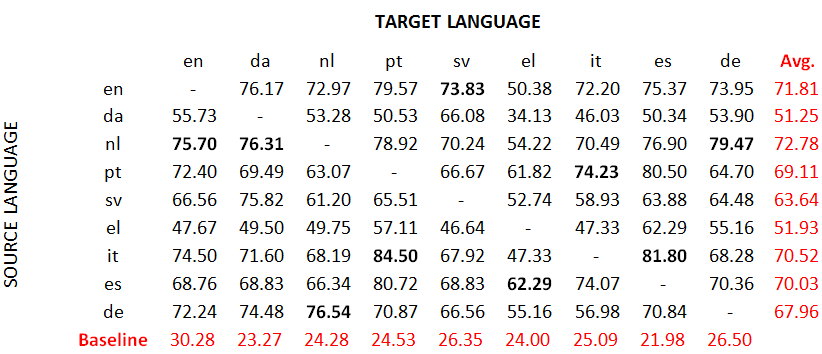
\includegraphics[scale=0.7]{Figures/TaggerPerformance}
\setlength{\tabcolsep}{3pt}
    \begin{tabular}{rccccccccccc}

          & \multicolumn{11}{c}{TARGET LANGUAGE} \\
          &       & en    & da    & nl    & pt    & sv    & el    & it    & es    & de    & \textbf{Avg.} \\
    \multicolumn{1}{c}{\multirow{10}[0]{*}{
	\begin{sideways}  
    SOURCE LANGUAGE
    \end{sideways}
}} & en    & -     & 76.17 & 72.97 & 79.57 & \textbf{73.83} & 50.38 & 72.20 & 75.37 & 73.95 & 71.81 \\
    \multicolumn{1}{c}{} & da    & 55.73 & -     & 53.28 & 50.53 & 66.08 & 34.13 & 46.03 & 50.34 & 53.90 & 51.25 \\
    \multicolumn{1}{c}{} & nl    & \textbf{75.70} & \textbf{76.31} & -     & 78.92 & 70.24 & 54.22 & 70.49 & 76.90 & \textbf{79.47} & 72.78 \\
    \multicolumn{1}{c}{} & pt    & 72.40 & 69.49 & 63.07 & -     & 66.67 & 61.82 & \textbf{74.23} & 80.50 & 64.70 & 69.11 \\
    \multicolumn{1}{c}{} & sv    & 66.56 & 75.82 & 61.20 & 65.51 & -     & 52.74 & 58.93 & 63.88 & 64.48 & 63.64 \\
    \multicolumn{1}{c}{} & el    & 47.67 & 49.50 & 49.75 & 57.11 & 46.64 & -     & 47.33 & 62.29 & 55.16 & 51.93 \\
    \multicolumn{1}{c}{} & it    & 74.50 & 71.60 & 68.19 & \textbf{84.50} & 67.92 & 47.33 & -     & \textbf{81.80} & 68.28 & 70.52 \\
    \multicolumn{1}{c}{} & es    & 68.76 & 68.83 & 66.34 & 80.72 & 68.83 & \textbf{62.29} & 74.07 & -     & 70.36 & 70.03 \\
    \multicolumn{1}{c}{} & de    & 72.24 & 74.48 & \textbf{76.54} & 70.87 & 66.56 & 55.16 & 56.98 & 70.84 & -     & 67.96 \\
    \multicolumn{1}{c}{} & \textbf{Baseline} & 30.28 & 23.27 & 24.28 & 24.53 & 26.35 & 24.00 & 25.09 & 21.98 & 26.50 &  \\
    \end{tabular}%


\caption{Tagger accuracy for each source--target language pair. The best tagger for each target language is shown in bold.}
\label{fig:taggerPerformance}
\end{table}

We evaluate each $Tagger(t)$ using $Data(t)$, and report the results
shown in Table~\ref{fig:taggerPerformance}. The average tagger
performance for each source language is also given. It turns out that
choosing Dutch (avg =72.78\%) as the source language rather than
English (avg=71.81\%) gives the best overall performance. The tagger
performance of each target language is much better than the baseline
that always picks the most frequent tag for each word.\footnote{For most of languages, the baseline is assigning ``Noun" for all words.} 

The Greek tagger performs poorly. From Table \ref{tbl:corpsizeVocSize}, Greek is the most morphologicaly complex language in this set, and has the smallest corpus size, two factors which partially explain why tagger performance for Greek is low regardless of whether Greek occupies the source or target language role. 

From Table~\ref{fig:taggerPerformance}, it seems that taggers perform better if the source and target language are in the same language family. For example, the top four source languages for Danish are English, Dutch, Swedish and German, and the top two source languages for Portuguese are Italian and Spanish. This confirms the intuition in adding language relatedness features in section \ref{featuresSec}. 

In chapter \ref{chap:uniTagger}, we also used English as the source language to build taggers for the same eight other languages. The only difference between these two experiments is that in chapter \ref{chap:uniTagger} experiment, we used Europarl \cite{europarl} data instead of JRC-Acquis. Table~\ref{tbl:acc2Models} compares the performance of each target language using English as the source language, for the two datasets. As mentioned before, Europarl is English oriented and not relevant for our experiment. Table~\ref{tbl:corpsizeVocSize} also compares the size of parallel
data having English as the source language, for both corpora. Given
that Europarl is much larger, higher performance is expected. However,
Table~\ref{tbl:acc2Models} shows a strong correlation between the two
experiments (Pearson's $r$ = 0.7).\footnote{The common rule of thumb interpretation for Pearson-correlation is as follows: $|r| > 0.7$ : very strong relationship, $> 0.4$ : strong relationship, $> 0.3$ : moderate relationship, $> 0.2$ : weak relationship, $>0.01$: no or negligible relationship. Negative r means a negative relationship.}
 
 
This suggests that, if we had as much data as Europarl for every language pair (not just English), we would expect all numbers in Table~\ref{fig:taggerPerformance} to improve substantially (not only the first row where English is the source language). 
%% Should we put the table showing size of europarl and acquis here ? 
%% Explain why the number is not as good as previous paper 
%% Explain why greek perform poorly 
%% 
\begin{table}
\small
\centering
    \begin{tabular}{lll}
    Language & JRC-Acquis & Europarl \\
    \hline
    da       &    76.2    &    85.6         \\ 
    nl       &    73.0    &    84.0         \\
    pt       &    79.6    &    86.3         \\
    sv       &    73.8    &    81.0         \\
    el       &    50.4    &    80.0         \\
    it       &    72.2    &    81.4         \\
    es       &    75.4    &    83.3         \\
    de       &    74.0    &    85.4         \\
    \hline
    Average  & 71.8       & 83.4            \\
    \end{tabular}
    \caption{Accuracy on JRC-Acquis and Europarl using English as the source language}
    \label{tbl:acc2Models}
\end{table}


\section{Source language prediction} 
\label{sec:sourceLanguagePrediction}
% SB: aren't models already predictive?
%% PC: Changed title accordingly
In this section, using features defined in section \ref{featuresSec} and the tagger performance shown in Table~\ref{fig:taggerPerformance}, we build a model that can predict the performance of the target language tagger given a source language. 

\subsection{Individual feature correlation}
Firstly, we want to determine the correlation of individual features with tagger performance. Table~\ref{tbl:individualFactorCor} shows the Pearson's correlation ($r$) and coefficient of determination ($r^2$) of each feature. The $r^2$ value can show the explanatory power, i.e., the extent to which the variance in tagger performance is "explained" by that factor. Significance shows the reliability of the calculation ($***$ means  
\emph{p-value} $< 0.001$, $**$ means \emph{p-value} $< 0.01$, $*$ means \emph{p-value}$ < 0.05$). 

\begin{table}
\centering
\small
    \begin{tabular}{lccc}
    Features & r & $r^2$ & Significance\\\hline
    Source Voc Size	& -0.613	&0.376 & $***$ \\
    Target Voc Size	& -0.202	& 0.041 & $*$ \\
    Corpus Size	& 0.620	& 0.385 & $***$ \\
    Language Relatedness	& 0.497	& 0.247 & $***$ \\
    Sentence Alignment Score & 	0.492	& 0.242 & $***$\\
    One-to-one Mapping Proportion	& 0.745	& 0.556& $***$\\
    Lexical Translation Entropy	& -0.590	& 0.348& $***$\\

    \end{tabular}
    \caption{Individual feature Pearson-correlation}
    \label{tbl:individualFactorCor}
\end{table}

Surprisingly, the one-to-one mapping proportion is very strongly correlated with tagger performance ($r=0.745)$. The value of $r^2 = 0.556$ means that 55.6\% of the variance in the tagger performance can be explained solely by this factor. The negative correlation for the lexical translation entropy model is easy to understand because lower entropy is better. The source language vocabulary size is highly negatively correlated, but that strong relationship is not found for the target language. This suggests that the model is not affected much by the target language, but prefers the source language to be morphologically simple.
%%%%%%%%%%%%%%%%% EXPLAIN WHY MODEL DOESN'T CARE ABOUT TARGET LANG ######


The corpus size factor is highly positively correlated too. This confirms the intuition that more data is better. This strong relationship, together with the negative morphological complexity factor, consolidates the explanation above about the poor performance of the tagger for Greek, where the availability of data is very limited, and where Greek has the richest morphology of any language considered.

%TODO : should mention why corpus size is so correlated ??? The data in the table is not so diffirence 

\subsection{Building a predictive model}
In this experiment we are interested in building a model that can predict the performance of a target language tagger given a source language. We fit all features into a multiple linear regression model. The $r^2$ value improved drastically to 0.74, meaning that 74\% of variance in tagger performance is explained by the factors we have identified.


\begin{table}
\centering
%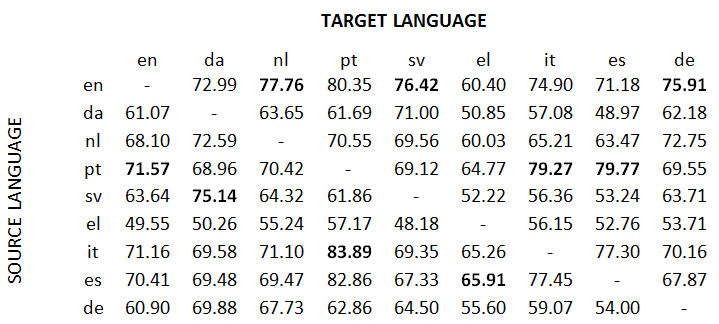
\includegraphics[scale=0.7]{Figures/Prediction}
    \begin{tabular}{rcccccccccc}

          & \multicolumn{10}{c}{TARGET LANGUAGE} \\

    \multicolumn{1}{c}{\multirow{10}[0]{*}{	
    \begin{sideways}  
    SOURCE LANGUAGE
    \end{sideways}
}} &       & en    & da    & nl    & pt    & sv    & el    & it    & es    & de \\
    \multicolumn{1}{c}{} & en    & -     & 72.99 & \textbf{77.76} & 80.35 & \textbf{76.42} & 60.40 & 74.90 & 71.18 & \textbf{75.91} \\
    \multicolumn{1}{c}{} & da    & 61.07 & -     & 63.65 & 61.69 & 71.00 & 50.85 & 57.08 & 48.97 & 62.18 \\
    \multicolumn{1}{c}{} & nl    & 68.10 & 72.59 & -     & 70.55 & 69.56 & 60.03 & 65.21 & 63.47 & 72.75 \\
    \multicolumn{1}{c}{} & pt    & \textbf{71.57} & 68.96 & 70.42 & -     & 69.12 & 64.77 & \textbf{79.27} & \textbf{79.77} & 69.55 \\
    \multicolumn{1}{c}{} & sv    & 63.64 & \textbf{75.14} & 64.32 & 61.86 & -     & 52.22 & 56.36 & 53.24 & 63.71 \\
    \multicolumn{1}{c}{} & el    & 49.55 & 50.26 & 55.24 & 57.17 & 48.18 & -     & 56.15 & 52.76 & 53.71 \\
    \multicolumn{1}{c}{} & it    & 71.16 & 69.58 & 71.10 & \textbf{83.89} & 69.35 & 65.26 & -     & 77.30 & 70.16 \\
    \multicolumn{1}{c}{} & es    & 70.41 & 69.48 & 69.47 & 82.86 & 67.33 & \textbf{65.91} & 77.45 & -     & 67.87 \\
    \multicolumn{1}{c}{} & de    & 60.90 & 69.88 & 67.73 & 62.86 & 64.50 & 55.60 & 59.07 & 54.00 & - \\

    \end{tabular}%

\caption{Predicted Tagger Accuracy for each source-target language pair. The best predicted tagger for each target language is in bold }
\label{fig:taggerPerformancePredicted}
\end{table}

We evaluate our model in a leave-one-out cross validation experiment. To build a predictive model for language $t$, we remove data in Table~\ref{fig:taggerPerformance} associated with $t$ and train the multiple linear regression model $model(t)$ on the remaining data. So, given source language $s$ and $(s-t)$ parallel data sets, $model(t)$ outputs the predicted performance of the tagger trained on $(s-t)$ parallel data sets. The predicted accuracy for each language pair is given in Table \ref{fig:taggerPerformancePredicted}. However, the correlation of the predicted value (Table \ref{fig:taggerPerformancePredicted}) with the original value (Table~\ref{fig:taggerPerformance}) is very high ($r=0.81$). 

We also build another predictive model based solely on monolingual features (morphology complexity and language relatedness). The intuition here is that, if we only have monolingual data and we are planning to build a tagger for target language $t$, what parallel data would we want to collect first? This monolingual model also shows a high correlation with the original table ($r=0.74$). If we only use language relatedness, the correlation is very weak ($r=0.13$), showing that language relatedness on its own is not effective at predicting the best source language.

The predicted best source language for each target language $t$ is the language predicted to produce the highest accuracy tagger. For example, from Table \ref{fig:taggerPerformancePredicted}, if we want to build a tagger for Danish (da), we will choose Swedish (sv) as the source language. Table~\ref{tbl:sourceLangPrediction} shows the source language prediction from models exploiting all features, and only monolingual features. The Fixed model always chooses Dutch (nl) as the source language, because Dutch gives the highest average accuracy (Table~\ref{fig:taggerPerformance}). The Oracle model always picks the best language, and gives the upper bound for the predictive model as a point of comparison. As expected, the model exploiting all features achieves a higher average accuracy than the monolingual model, which nevertheless still outperforms Fixed. With respect to the oracle upperbound, and Fixed baseline, the error rate reduction for the monolingual and all features models is 10.9\% and 52.3\%, respectively, showing the effectiveness of using a predictive model.


\begin{table}
\small
\centering
    \begin{tabular}{cccc|c}
    Target language & All features & Monolingual features & Fixed& Oracle\\\hline
    en              & pt (72.40)          & \textbf{nl (75.70)} & \textbf{nl (75.70)}& nl (75.70) \\ 
    da              & sv  (75.82)          & en (76.17)  & \textbf{nl (76.31)} &  nl (76.31)\\
    nl              & \textbf{en  (72.97)}              & \textbf{en (72.97)}&  - & de (76.54)\\
    pt              & \textbf{it  (84.50)}           & es (80.72)& nl (78.92
) & it (84.50)\\
    sv              & \textbf{en  (73.83)}               & \textbf{en (73.83)} & nl (70.24) & en (73.83)\\
    el              & \textbf{es  (62.29)}            & en (50.38)& nl (54.22) & es  (62.29) \\
    it              & \textbf{pt  (74.23)}          & es (74.07) & nl (70.49) & pt  (74.23) \\
    es              & \textbf{pt   (80.50)}          & \textbf{pt (80.50)}  & nl (76.90) & it (81.80)\\
    de              & en  (73.95)         & en (73.95)  & \textbf{nl (79.47)} & nl (79.47)\\ \hline
    Average         & \textbf{ \phantom{xx (}74.50\phantom{)} }     & \phantom{xx (}73.14\phantom{)}& \phantom{xx (}72.78\phantom{)} & \phantom{xx (}76.07\phantom{)}
    \end{tabular}
    \caption{Best source language prediction (and corresponding tagger performance) for models exploiting all features, only monolingual features, and a fixed source language, as well as an oracle model that always picks the best language. The best (non-oracle) source language and accuracy for each target language is shown in bold.}
    \label{tbl:sourceLangPrediction}
\end{table}

% MULTIPLE SOURCE LANGUAGES 
\section{Multiple Source Languages}
\label{sec:multipleSourceLanguages}


\begin{figure}
\centering
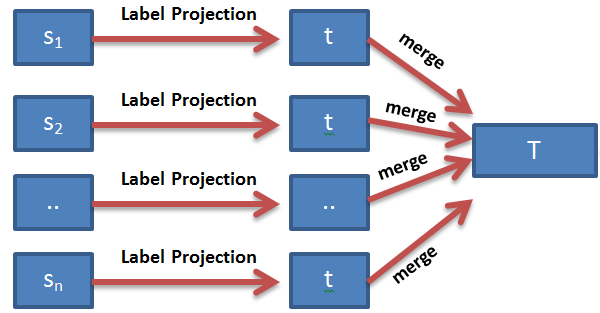
\includegraphics[scale=0.7]{Figures/multiSource}
\caption{Combining multiple source language to produce single file }
\label{fig:multipleSource}
\end{figure}

%% PC: Need to update notation in Figure to match text.
%% LD: Done
In this section we combine information from multiple source languages
to build a single target language tagger. We take a simple approach as shown in Figure \ref{fig:multipleSource}. Each $s_i$ is a
tagged corpus for source language $i$. POS tags are then projected to
the target language side $t$ for each corpus. We merge all of these
partially-tagged target language corpora (in which unaligned words are
untagged) to form $T$. Because the JRC-Acquis corpus consists
  of translations of documents into multiple languages, in many cases
  the same target language sentence occurs in the parallel corpus for
  multiple source languages. In this preliminary approach to combining
  information from multiple source languages, we simply treat these as
  different target language sentences because the sentences are
  aligned with different source languages, they might contain
  different partial tag information.  
  
We build the target language tagger from $T$ by adapting the method from chapter
\ref{chap:uniTagger} (Universal Tagger). The typical steps for this method are (1) tag the source language, (2) project labels from the source to target
language, (3) build the seed model, and (4) apply self-training with
revision to produce the final model. Here we simply start from step
(3) and build the seed model from $T$.

 \begin{table}
 \centering
     \begin{tabular}{clllllll}
     Language    & 1 best & 2 best      & 3 best       & 4 best       & 5 best       & 6 best       & 7 best      \\\hline
     en      &    75.70    &    76.36 &    76.66 &    77.17 &    76.36 &    77.06 &    \textbf{78.16} \\
     da      &    76.31    &    78.06 &    78.40 &    \textbf{83.35} &    82.45 &    82.60 &    82.43 \\
     nl      &    76.54    &    76.82 &    76.17 &    76.03 &    80.00 &    \textbf{81.60} &    81.45 \\
     pt      &    84.50    &    83.84 &    84.91 &    84.79 &    85.00 &    \textbf{85.46} &    84.24 \\
     sv      &    73.83    &    74.33 &    74.65 &    74.49 &    74.10 &    74.51 &    \textbf{76.66 }\\
     el      &    62.29    &    66.90 & \textbf{ 70.23} &    67.93 &    67.22 &    67.03 &    67.69 \\
     it      &    74.23    &    77.28 &    \textbf{78.71} &    78.47 &    78.47 &    78.03 &    76.05 \\
     es      &    81.80    &    81.89 &    82.53 &    \textbf{82.76} &    82.13 &    82.21 &    82.64 \\
     de      &  \textbf{  79.47}    &    79.35 &    79.28 &    78.79 &    77.92 &    77.88 &    77.35 \\\hline
     Average &    76.07    &    77.20 &    77.95 &    78.20 &    78.18 &    78.49 &    \textbf{78.52} \\
     Run time(s) & 352 & 444 & 741 & 1025 & 1648 & 2790 & 3297
     \end{tabular}    \caption{Tagger performance when combine multiple source language and performance of Portuguese languages measured in seconds. The best system are in bold }
     \label{tbl:multipleSource}
 \end{table}

%\begin{table}
%\small
%\centering
%    \begin{tabular}{lrrrr}
%    Language    & 1-best       & 3-best         & 5-best         &  7-best      \\
%\hline
%    en      &    75.70         &    76.66       &    76.36       &     \textbf{78.16} \\
%    da      &    76.31         &    78.40       & \textbf{82.45} &     82.43 \\
%    nl      &    76.54         &    76.17       &    80.00       &     \textbf{81.45} \\
%    pt      &    84.50         &    84.91       &    \textbf{85.00}       &     84.24 \\
%    sv      &    73.83         &    74.65       &    74.10       &     \textbf{76.66 }\\
%    el      &    62.29         & \textbf{70.23} &    67.22       &     67.69 \\
%    it      &    74.23         & \textbf{78.71} &    78.47       &     76.05 \\
%    es      &    81.80         &    82.53       &    82.13       &     \textbf{82.64} \\
%    de      &  \textbf{79.47}  &    79.28       &    77.92       &     77.35 \\
%\hline
%    Average &    76.07         &    77.95       &    78.18 &     \textbf{78.52} \\
%    %% Run time(s) & 352 & 741 & 1648 & 3297\\
%    \end{tabular}
%    \caption{Tagger accuracy when combining the 1-, 3-, 5-, and 7-best
%      source languages. The best system for each target language is shown in
%      bold.}
%    \label{tbl:multipleSource}
%\end{table}

In these experiments we assume that when building a tagger for a
target language we have access to all other source languages. Table
\ref{tbl:multipleSource} shows accuracy when combining information
from the \mbox{1-,} \mbox{2-,} \mbox{3-,} to 7-best source languages
(where the best source language is determined by an oracle). As more
source languages are added, the average accuracy increases, although
there is some variation for individual languages. Nevertheless, these
findings show that the method described in chapter \ref{chap:uniTagger} is robust and can be substantially improved by combining information from multiple source
languages. There is, however, a trade-off between accuracy and
efficiency, with taggers built from multiple source languages
generally being slower.
The memory and running time is $O(nlogn)$ with the amount of data $n$. Table \ref{tbl:multipleSource} also shows the running time for
 Portuguese on each combination. We run our experiment on a 16 cores Intel Xeon 2.53 GHz server with 24GB RAM. 
%% We assume that when building tagger for target language we have all
%% other source languages available. Table \ref{tbl:multipleSource} show
%% the tagger performance when combining the single best, 2 best, 3 best,
%% 4 best, 5 best, 6 best and 7 best source languages. Table
%% \ref{tbl:multipleSource} confirms the robustness of \cite{Duong:2013}
%% method. As more data are added, it introduced more noise, however, in
%% general, the model handles it well as average performance
%% increased. The memory and running time is $O(nlogn)$ with the amount
%% of data $n$. Table \ref{tbl:multipleSource} shows the running time for
%% Portuguese on each combination. We ran our experiment on a Intel(R)
%% Xeon(R) 2.53GHz server with 24GB RAM . The running time is measured in
%% seconds. Therefore, as the trade-off between performance and
%% computational complexity, we would prefer using just 4 best
%% systems. Out of 9 languages, using up to 4 best source language give
%% us the best performance for 5 languages. On average, 4 best option
%% achieves competitive result but remain fast. For the best accuracy, we
%% would use all possibles source languages.

\section{Summary of Contributions}

In this chapter, we investigated the problem of choosing the best
source language(s) to use in unsupervised multilingual POS tagging based
on tag projection in parallel corpora. We have shown that our predictive model can select a source language --- based on only monolingual features of the source and
target languages --- that improves tagger accuracy compared to
choosing the single best (overall) source language. However, if
parallel data is available, our predictive model is able to leverage
this to select a more appropriate source language and obtain further
improvements in accuracy. Finally, we showed that if multiple source
languages are available, even better accuracy can be obtained by
combining information from just those sources that are selected by our model. A synopsis of the process for building a tagger for language $S$ is described in Figure \ref{fig:cheatSheet}. That is, if we do not have any parallel data, we would use a monolingual model to predict the best source language $T$ and collect $S-T$ parallel data sets. If multiple parallel data sets are available and we have time, the best solution is just to combine all source languages to produce the single best tagger. If we do not have time, just combine $n$-best source languages in the order defined by \textit{all features model} gave the comparable accuracy but stay fast. 

\begin{figure}
\centering
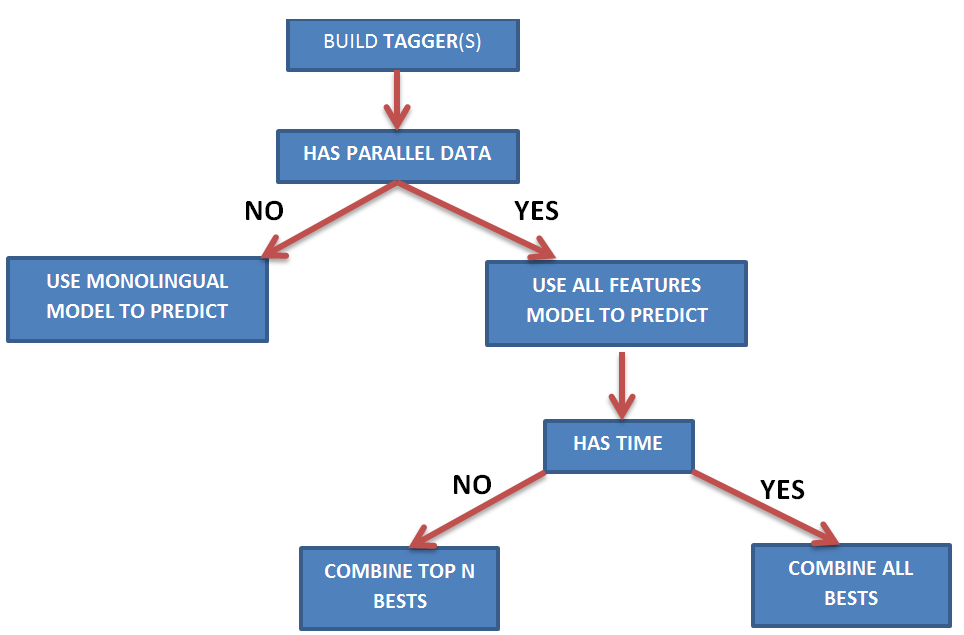
\includegraphics[scale=0.5]{Figures/cheatSheet}
\caption{Instruction for building tagger for target language $S$}
\label{fig:cheatSheet}
\end{figure}

In future work, we would like to apply the methods described in this
paper for identifying ``good'' source languages for other multilingual
NLP tasks which exploit parallel data to transfer annotations between
languages, including grammar induction, parsing, and morphological
analysis. We further intend to expand our experiments to consider more
source and target languages. We also would like to investigate more methods for combining different source languages. Currently, we ignore cross-language sentences and concatenate them without any further processing. This resource can be very valuable since we have the POS information from all other languages for each individual sentence. Thus, we can combine and produce more accurate tagged sentences which will serve as better training data for the POS tagger. 
%% To the best of our knowledge, we are first quantifying the question
%% ``which is the best source language for a target POS tagger". Our
%% predicting model which build just on monolingual features has proved
%% to be useful and very easy to build. We also gave thoroughly analysis
%% about the performance of multiple source languages. In summary, if we
%% don't have any parallel data, we will use our monolingual predicting
%% model to predict the source language. If we have parallel data, the
%% best thing to do is just combining all of them. In the future, we
%% would like to testify our methods on other multilingual natural
%% language processing(NLP) tasks which exploiting parallel data to copy
%% annotated label from source to target language. These tasks might be,
%% grammar induction, parsing, morphology analysis etc. We also would
%% like to expand this experiment to other languages. This way, we can
%% make a bigger matrix ranking source language for each target language.
